\documentclass[11pt,english]{article}

%%%%%%%%%%%%%%%%%%%%%%%%%%%%%%%%%%%%%%%%%%%%%%%%%%%%%%%%%%%
% Packages
%%%%%%%%%%%%%%%%%%%%%%%%%%%%%%%%%%%%%%%%%%%%%%%%%%%%%%%%%%%

% Package imports are stored in assets/base-packages.tex
% Packages specific to this pset can be imported here.

\listfiles
% paper size & margins
\usepackage{fullpage}
\usepackage[showframe=false,margin=1in]{geometry}
\parindent=0pt

% font management
\usepackage{relsize}
\usepackage[T1]{fontenc} % for properly hyphenating words with accented chars
\usepackage[latin1]{inputenc}
\usepackage{babel}

% figure management
\usepackage{epsfig}
\usepackage{graphicx}
\usepackage{wrapfig}
\usepackage{subfig}
%\usepackage{subfigure}
\usepackage[belowskip=0pt,aboveskip=0pt,font=small]{caption}
%\usepackage{subcaption}
\setlength{\intextsep}{7pt plus 0pt minus 0pt}

% math
\usepackage{amsmath, amsthm, amssymb}
%\usepackage{amstext}
\usepackage{textcomp}
\usepackage{stmaryrd}
\usepackage{upgreek}
\usepackage{bm}
\usepackage{cases}
\usepackage{mathtools}

% assorted
\usepackage{url}
\usepackage{breakurl}
\usepackage[colorlinks=true]{hyperref}
\usepackage{xspace}
\usepackage{comment}
\usepackage{color}
\usepackage{afterpage}
\usepackage[normalem]{ulem}
\usepackage{enumitem}



%%%%%%%%%%%%%%%%%%%%%%%%%%%%%%%%%%%%%%%%%%%%%%%%%%%%%%%%%%%
% Shortcuts
%%%%%%%%%%%%%%%%%%%%%%%%%%%%%%%%%%%%%%%%%%%%%%%%%%%%%%%%%%%
\usepackage{assets/mysymbols}
%%% load AMS-Latex Package
\usepackage{amsmath,amsfonts}
\usepackage{amsthm,amssymb,amsopn}
\usepackage{bm} % bold symbol
\usepackage{bbm}

% define fonts
\newcommand{\vct}[1]{\boldsymbol{#1}} % vector
\newcommand{\mat}[1]{\boldsymbol{#1}} % matrix

%%%% Special math symbols
\newcommand{\field}[1]{\mathbb{#1}}
\newcommand{\R}{\field{R}} % real domain
\newcommand{\C}{\field{C}} % complex domain
\newcommand{\F}{\field{F}} % functional domain
%\newcommand{\T}{^{\top}\!\!} % transpose
\newcommand{\T}{^{\textrm T}} % transpose
\newcommand{\TN}{^{-\textrm T}} % transpose
\newcommand{\Lagr}{\mathcal{L}}


%%% define constant
\newcommand{\cst}[1]{\mathsf{#1}}

%% operator in linear algebra, functional analysis
\newcommand{\inner}[2]{#1\cdot #2}
%\newcommand{\norm}[1]{\|#1\|}
\newcommand{\twonorm}[1]{\|#1\|_2^2}
% operator in functios, maps such as M: domain1 --> domain 2
\newcommand{\Map}[1]{\mathcal{#1}}

% operator in probability: expectation, covariance,
\newcommand{\ProbOpr}[1]{\mathbb{#1}}
% independence
\newcommand\independent{\protect\mathpalette{\protect\independenT}{\perp}}
\def\independenT#1#2{\mathrel{\rlap{$#1#2$}\mkern2mu{#1#2}}}
% conditional independence
\newcommand{\cind}[3]{{#1} \independent{#2}\,|\,#3}
% conditional expectation
\newcommand{\cndexp}[2]{\ProbOpr{E}\,[ #1\,|\,#2\,]}

% operator in optimization
%\DeclareMathOperator{\argmax}{arg\,max}
%\DeclareMathOperator{\argmin}{arg\,min}
%\newcommand{\todo}[1]{{\color{red}#1}}


% environment
\newtheorem{thm}{Theorem}

\newcommand{\eat}[1]{}

\newcommand{\hide}[1]{}
%\newcommand{\solution}{{\Large \vspace{5mm} \textbf{{\color{red}Solution:}}\newline\newline}}

\newcommand{\diff}{\mathop{}\!\mathrm{d}}
\newcommand{\Vop}{\textrm{T}}
\newcommand{\norminf}[1]{\norm{#1}_\infty}

% definitions for PS4
\newcommand{\vecy}{\ensuremath{\mathbf{y}}\xspace}
\newcommand{\vecx}{\ensuremath{\mathbf{x}}\xspace}
\renewcommand{\argmax}{\operatornamewithlimits{argmax}}
\newcommand{\startsym}{\mbox{\scriptsize \texttt{<s>}}\xspace}
\newcommand{\stopsym}{\mbox{\scriptsize \texttt{</s>}}\xspace}
\newcommand{\best}{\ensuremath{\mathit{best}}\xspace}
\newcommand{\bestuptoi}{\ensuremath{\texttt{best}_{\leq i}}\xspace}
\newcommand{\bestuptot}{\ensuremath{\texttt{best}_{\leq t}}\xspace}
\newcommand{\completed}{\ensuremath{\texttt{comp}}\xspace}
\newcommand{\toptop}{\operatornamewithlimits{\mathbf{top}}}
\newcommand{\tuple}[1]{\ensuremath{\langle {#1} \rangle}}
\newcommand{\xuptot}{\ensuremath{\mathit{x}_{\leq t}}\xspace}


\renewcommand{\hide}[1]{}

%%%%%%%%%%%%%%%%%%%%%%%%%%%%%%%%%%%%%%%%%%%%%%%%%%%%%%%%%%%
% Title / Author
%%%%%%%%%%%%%%%%%%%%%%%%%%%%%%%%%%%%%%%%%%%%%%%%%%%%%%%%%%%
\begin{document}
\title{CS 4644/7643: Deep Learning\\
Spring 2022 \\
Problem Set 2}

% NOTE: Any changes to instructor, TAs, or piazza link should be done in the file below
\author{Instructor: Zsolt Kira \\
TAs: Bhavika Devnani, Jordan Rodrigues, Mandy Xie, \\Yanzhe Zhang, Amogh Dabholkar, Ahmed Shaikh, \\ Ting-Yu Lan, Anshul Ahluwalia, Aditya Singh, Yash Jakhotiya\\
\\
Discussions: \url{https://piazza.com/gatech/spring2022/cs46447643a}}
\date{Due: 11:59pm, February 23, 2022}
\maketitle


\paragraph*{Instructions}
\begin{enumerate}
\item We will be using Gradescope to collect your assignments.  Please read the following instructions for submitting to Gradescope carefully!
     \begin{itemize}
          \item
               For the \textbf{HW2 Writeup} component on Gradescope, you could upload one single PDF containing the answers to all the theory questions and the report for the coding problems. \textbf{However, the solution to each problem/subproblem must be on a separate page. When submitting to Gradescope, please make sure to mark the page(s) corresponding to each problem/sub-problem.} Likewise, the pages of the report must also be marked to their corresponding subproblems.
          \item
               For the \textbf{HW2 Code Part 1 and Part 2} components on Gradescope, 
               please use the \texttt{collect\_submission.py} script provided and upload the resulting zip files to each Gradescope section respectively. Please make sure you have saved the most recent version of your codes.
          \item
               Note: This is a large class and Gradescope's assignment segmentation features are essential.
               Failure to follow these instructions may result in parts of your assignment not being graded.
               We will not entertain regrading requests for failure to follow instructions.
     \end{itemize}

\item
     \LaTeX'd solutions are strongly encouraged (solution template available in the zip file in HW2 under the Assignments tab on Canvas),
     but scanned handwritten copies are acceptable.
     Hard copies are \textbf{not} accepted.


\item We generally encourage you to collaborate with other students.

You may talk to a friend,
discuss the questions and potential directions for solving them. However, you need to write
your own solutions and code separately, and \emph{not} as a group activity.
Please list the students you collaborated with. \\ \\
\end{enumerate}
\newpage

%%%%%%%%%%%%%%%%%%%%%%%%%%%%%%%%%%%%%%%%%%%%%%%%%%%%%%%%%%%
% Body
%%%%%%%%%%%%%%%%%%%%%%%%%%%%%%%%%%%%%%%%%%%%%%%%%%%%%%%%%%%

\section{Collaborators [0.5 points]}

Please list your collaborators and assign this list to the corresponding section of the outline on Gradescope. If you don't have any collaborators, please write 'None' and assign it to the corresponding section of the Gradescope submission regardless.


\section{Gradient Descent}
\begin{enumerate}[start]

\item
\textbf{[3 points]}

We often use iterative optimization algorithms such as Gradient Descent to
find $\mathbf{w}$ that minimizes a loss function $f(\mathbf{w})$. Recall that in gradient descent,
we start with an initial value of $\mathbf{w}$ (say $\mathbf{w}^{(1)}$) and iteratively take a step in the direction
of the negative of the gradient of the objective function \ie
%
\begin{equation}
\mathbf{w}^{(t+1)} = \mathbf{w}^{(t)} - \eta\nabla f(\mathbf{w}^{(t)})
\end{equation}
%
for learning rate $\eta > 0$.

In this question, we will develop a slightly deeper understanding of this update rule, in particular for 
minimizing a convex function $f(\mathbf{w})$. Note: this analysis will not directly carry over to training neural networks 
since loss functions for training neural networks are typically not convex, but this will (a) develop intuition 
and (b) provide a starting point for research in non-convex optimization (which is beyond the scope of this class). 


Recall the first-order Taylor approximation of $f$ at $\mathbf{w}^{(t)}$:
%
\begin{align}\label{first-order-approx}
f(\mathbf{w}) \approx f(\mathbf{w}^{(t)}) + \langle \mathbf{w}-\mathbf{w}^{(t)},
\nabla f(\mathbf{w}^{(t)}) \rangle
\end{align}
%
When $f$ is convex, this approximation forms a lower bound of $f$, \ie 
\begin{align}
f(\mathbf{w}) \ge 
\underbrace{
f(\mathbf{w}^{(t)}) + \langle \mathbf{w}-\mathbf{w}^{(t)}, 
\nabla f(\mathbf{w}^{(t)}) \rangle
}_{\text{affine lower bound to $f(\cdot)$}}
 \quad \forall \mathbf{w}
\end{align}
%

Since this approximation
is a `simpler' function than $f(\cdot)$, we could consider minimizing the approximation instead of $f(\cdot)$.
Two immediate problems: (1) the approximation is affine (thus unbounded from below) and
(2) the approximation is faithful for $\mathbf{w}$ close to $\mathbf{w}^{(t)}$.
To solve both problems, we add a squared $\ell_2$ \emph{proximity term} to the approximation minimization:
%
\begin{equation}
\argmin_\mathbf{w}
\underbrace{
f(\mathbf{w}^{(t)}) + \langle \mathbf{w}-\mathbf{w}^{(t)}, \nabla f(\mathbf{w}^{(t)}) \rangle
}_{\text{affine lower bound to $f(\cdot)$}}
+
\underbrace{
\frac{\lambda}{2}
}_{\text{trade-off}}
\underbrace{
\norm{\mathbf{w} - \mathbf{w}^{(t)}}^2
}_{\text{proximity term}}
\end{equation}
%

Notice that the optimization problem above is an unconstrained quadratic programming problem,
meaning that it can be solved in closed form (hint: gradients).

What is the solution $\mathbf{w}^*$ of the above optimization?
What does that tell you about the gradient descent update rule?
What is the relationship between $\lambda$ and $\eta$?


\item
\textbf{[4 points]}

Let's prove a lemma that will initially seem devoid of the rest of the analysis but will come 
in handy in the next sub-question when we start combining things. 
Specifically, the analysis in this sub-question holds for any $\mathbf{w}^{\star}$, but in the next sub-question  
we will use it for $\mathbf{w}^{\star}$ that minimizes $f(\mathbf{w})$. 

Consider a sequence of vectors $\mathbf{v}_1, \mathbf{v}_2, ..., \mathbf{v}_T$, 
and an update equation of the form $\mathbf{w}^{(t+1)} = \mathbf{w}^{(t)} - \eta\mathbf{v}_{t}$ 
with $\mathbf{w}^{(1)} = 0$. 
Show that: 

\begin{equation}
\sum_{t=1}^T \langle \mathbf{w}^{(t)}-\mathbf{w}^{\star}, \mathbf{v}_t \rangle \leq
\frac{\norm{\mathbf{w}^{\star}}^2}{2\eta} + \frac{\eta}{2} \sum_{t=1}^T \norm{\mathbf{v}_t}^2
\end{equation}

\item
\textbf{[4 points]}

Now let's start putting things together and analyze the convergence rate of gradient descent \ie
how fast it converges to $\mathbf{w}^\star$. For this question, assume that $f$ is convex and $\rho$-Lipschitz. A function that is $\rho$-Lipschitz is one where the norm of its gradient is bounded by $\rho$, i.e. $\norm{\nabla f(\mathbf{w})} \leq \rho$.

First, show that for $\mathbf{\bar w} = \frac{1}{T} \sum_{t=1}^T \mathbf{w}^{(t)}$

\begin{equation}
f(\mathbf{\bar w}) - f(\mathbf{w}^\star) \leq \frac{1}{T} \sum_{t=1}^T
\langle \mathbf{w}^{(t)}-\mathbf{w}^{\star}, \nabla f(\mathbf{w}^{(t)}) \rangle
\end{equation}

Next, use the result from part $2$, with upper bounds $B$ and $\rho$ for
$\norm{\mathbf{w}^\star}$ and $\norm{\nabla f(\mathbf{w}^{(t)})}$
respectively and show that for fixed $\eta = \sqrt{\frac{B^2}{\rho^2T}}$,
the convergence rate of gradient descent is $\mathcal{O}(1/\sqrt{T})$
\ie the upper bound for $f(\mathbf{\bar w}) - f(\mathbf{w}^\star)$
$\propto$ $\frac{1}{\sqrt{T}}$.

\end{enumerate}


\section{Estimating Hessians [Extra credit for 4644]}
\begin{enumerate}[resume]

\item
\textbf{[6 points]}

Optimization is an extremely important part of deep learning. In the previous question, we explored gradient descent, which uses the direction of maximum change to minimize a loss function. However, gradient descent leaves a few questions unresolved -- how do we choose the learning rate $\eta$? If $\eta$ is small, we will take a long time to reach the optimal point; if $\eta$ is large, it will oscillate between one side of the curve and another. So what should we do? 

One solution is to use Hessians, which is a measure of curvature, or the rate of change of the gradients. Intuitively, if we knew how steep a curve were, we would know how fast we should move in a given direction. This is the intuition behind second-order optimization methods such as Newton's method. 

Let us formally define a Hessian matrix $\mathbf{H}$ of a function $f$ as a square $n \times n$ matrix containing all second partial derivatives of $f$, i.e.:

\[ \mathbf{H} = 
\begin{bmatrix}
    \frac{\partial^2 f}{\partial x_1^2} & \frac{\partial^2 f}{\partial x_1 \partial x_2} & \dots  & \frac{\partial^2 f}{\partial x_1 \partial x_n} \\
    \frac{\partial^2 f}{\partial x_2 \partial x_1} & \frac{\partial^2 f}{\partial x_2^2 } & \dots  & \frac{\partial^2 f}{\partial x_2 \partial x_n} \\
    \vdots & \vdots  & \ddots & \vdots\\
    \frac{\partial^2 f}{\partial x_n \partial x_1} & \frac{\partial^2 f}{\partial x_n \partial x_2} & \dots  & \frac{\partial^2 f}{\partial x_n^2} \\
\end{bmatrix}
\]

Recall the second-order Taylor approximation of $f$ at $\mathbf{w}^{(t)}$:
%
\begin{align}
f(\mathbf{w}) \approx f(\mathbf{w}^{(t)}) + \langle \mathbf{w}-\mathbf{w}^{(t)},
\nabla f(\mathbf{w}^{(t)}) \rangle + \frac{1}{2}(\mathbf{w}-\mathbf{w}^{(t)})^\top
\mathbf{H} (\mathbf{w}-\mathbf{w}^{(t)})
\end{align}

\begin{enumerate} 
\item What is the solution to the following optimization problem? %$\mathbf{w}^*$ of the above optimization?
\begin{align}
    \argmin_\mathbf{w}
    \left[
    %\underbrace{
    f(\mathbf{w}^{(t)}) + \langle \mathbf{w}-\mathbf{w}^{(t)},
    \nabla f(\mathbf{w}^{(t)}) \rangle + \frac{1}{2}(\mathbf{w}-\mathbf{w}^{(t)})^\top
    \mathbf{H} (\mathbf{w}-\mathbf{w}^{(t)})
    %}_{\text{second-order approximation of $f(\cdot)$}}
    \right]
\end{align}
What does that tell you about how to set the learning rate $\eta$ in gradient descent?
\end{enumerate}

Now that we've derived Netwon's update algorithm, we should also mention that there is a catch to using Newton's method. Newton's method requires us to 1) calculate $\mathbf{H}$, and 2) invert $\mathbf{H}$. Having to compute a Hessian is expensive; $\mathbf{H}$ is massive and we would also have to figure out how to store it. 


\begin{enumerate}[resume] 
\item Consider an MLP with 3 fully-connected layers, each with 50 hidden neurons, except for the output layer, which represents 10 classes. We can represent the transformations as 
$\mathbf{x} \in \mathbb{R}^{50} \longrightarrow 
\mathbf{h}^{(1)} \in \mathbb{R}^{50} \longrightarrow 
\mathbf{h}^{(2)} \in \mathbb{R}^{50} \longrightarrow
\mathbf{s} \in \mathbb{R}^{10}$. 
Assume that $\mathbf{x}$ does not include any bias feature appended to it. 
How many parameters are in this MLP? What is the size of the corresponding Hessian?
\end{enumerate}

% \begin{enumerate} 
% \item  $\Delta \mathbf{w} = -\eta \mathbf{H}_f^{-1} \nabla f$. (Hint: Consider a Taylor series approximation).
% \end{enumerate}

Rather than store and manipulate the Hessian $\mathbf{H}$ directly, we will 
%Rather than computing $\mathbf{H}^{-1} \nabla f$ directly, 
instead focus on being able to compute the result of a Hessian-vector product 
$\mathbf{H}\mathbf{v}$, where $\mathbf{v}$ is an arbitrary vector. 
Why? Because in many cases one does not need the full Hessian but only $\mathbf{H}\mathbf{v}$.
Computing $\mathbf{H}\mathbf{v}$ is a core building block for computing a number of quantities including $\mathbf{H}^{-1} \nabla f$ (hint, hint). 
You will next show a surprising result that it is 
possible to `extract information from the Hessian', specifically to compute 
the Hessian-vector product 
%This allows information to be extracted from the Hessian 
without ever explicitly calculating or storing the Hessian itself!

Consider the Taylor series expansion of the gradient operator about a point in weight space: 
\begin{align}\label{second-order-expantion}
    \nabla_\mathbf{w} (\mathbf{w} + \Delta \mathbf{w}) = \nabla_\mathbf{w} (\mathbf{w}) + \mathbf{H} \Delta \mathbf{w} + O(|| \Delta \mathbf{w} ||^2)
\end{align}

where $\mathbf{w}$ is a point in weight space, $\Delta \mathbf{w}$ is a perturbation of $\mathbf{w}$, $\nabla_w$ is the gradient, and $\nabla_\mathbf{w} (\mathbf{w} + \Delta \mathbf{w})$ is the gradient of $f$ evaluated at $\mathbf{w} + \Delta \mathbf{w}$.

If you have difficulty understanding this expression above, consider starting with Eqn \ref{first-order-approx}, replacing 
$\mathbf{w} - \mathbf{w}^{(t)}$ with $\Delta \mathbf{w}$ and $f(\cdot)$ with $\nabla_\mathbf{w}(\cdot)$. 


% Add more explanation to 4(b). What specifically should they report? Something like “express Hv in terms of gradients of blah”. Basically, what should they try to get on the RHS. And why might it be an approximation.

\begin{enumerate}[resume] 
\item 
Use Eqn \ref{second-order-expantion} to derive a numerical approximation of $\mathbf{H}\mathbf{v}$ (in terms of $\nabla_{\mathbf{w}}$). 

Hint: Consider choosing $\Delta \mathbf{w} = r\mathbf{v}$, where $\mathbf{v}$ is a vector and $r$ is a small number.

\end{enumerate}
 
This approximation you derived above is susceptible to numerical instability. We would like a method that is free of these numerical issues and is exact instead of an approximation. To that end, let's now define a useful operator, known as the $\mathcal{R}$-operator. The $\mathcal{R}$-operator with respect to $\mathbf{v}$ is defined as: 
\begin{align}
    \mathcal{R}_{\mathbf{v}}\{f(\mathbf{w})\} = \frac{\partial}{\partial r} f (\mathbf{w} + r\mathbf{v})\Bigr\rvert_{r = 0}
\end{align}


%  In 4(c), first define the operator. Provide it a name (“R-operator”). Ask them to prove maybe 1 or 2 properties of R operators from here (https://cswhjiang.github.io/2015/10/13/Roperator/). Then ask them how they can use the R operator to compute Hv exactly.
 
\begin{enumerate}[resume] 

\item The $\mathcal{R}$-operator has many useful properties. Let's first prove some of them. Show that: 

\begin{center}
    $\mathcal{R}_{\mathbf{v}}\{cf(\mathbf{w})\}$ = $c\mathcal{R}_{\mathbf{v}}\{f(\mathbf{w})\}$ \qquad \qquad \qquad \qquad  [\text{Linearity under scalar multiplication}]
    

    $\mathcal{R}_{\mathbf{v}}\{f(\mathbf{w})g(\mathbf{w})\}$ = $\mathcal{R}_{\mathbf{v}}\{f(\mathbf{w})\}g(\mathbf{w}) + f(\mathbf{w})\mathcal{R}_{\mathbf{v}}\{g(\mathbf{w})\}$ \quad [\text{Product Rule of R-operators}]

\end{center}


\item Now, instead of numerically approximating $\mathbf{H}\mathbf{v}$, use the $\mathcal{R}$-operator to derive an equation to exactly calculate $\mathbf{H}\mathbf{v}$.

\item Explain how might you implement $\mathbf{H}\mathbf{v}$ in MLPs if you already have access to an auto-differentiation library. 
\end{enumerate}

\end{enumerate}


\section{Automatic Differentiation}
\begin{enumerate}[resume]

\item
\textbf{[4 points]}

In practice, writing the closed-form expression of the derivative of
a loss function $f$ w.r.t. the parameters of a deep neural network is hard
(and mostly unnecessary) as $f$ becomes complex. Instead, we define
computation graphs and use the automatic differentiation algorithms (typically backpropagation) to compute
gradients using the chain rule. For example, consider the expression

\begin{equation}
f(x, y) = (x+y)(y+1)
\end{equation}

Let's define intermediate variables $a$ and $b$ such that

\begin{equation}
a = x + y
\end{equation}
%
\begin{equation}
b = y + 1
\end{equation}
%
\begin{equation}
f = a \times b
\end{equation}
A computation graph for the ``forward pass'' through $f$ is shown in \figref{fig:graph}. 

\begin{figure}[h]
  \centering
    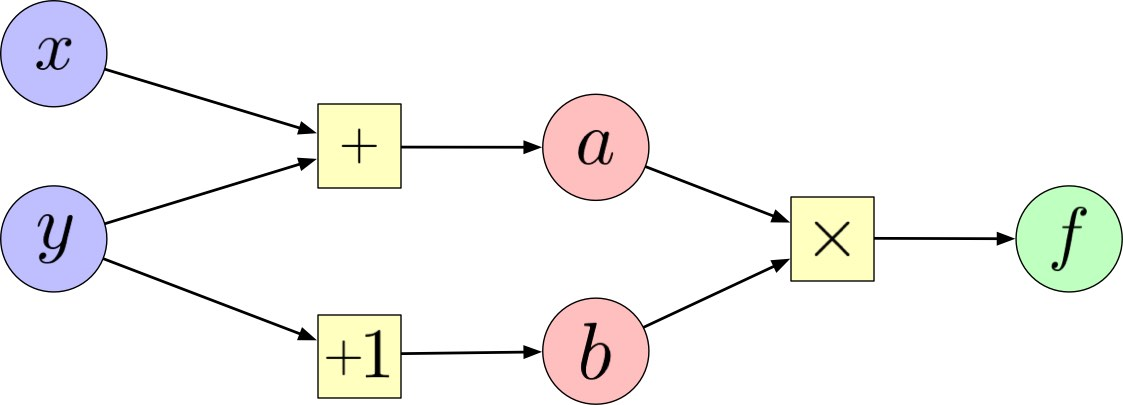
\includegraphics[width=0.5\textwidth]{assets/comp_graph_example.jpg}
    \caption{}
    \label{fig:graph}
\end{figure}

We can then work backwards and compute the derivative of $f$ w.r.t. each
intermediate variable ($\frac{\del f}{\del a}$, $\frac{\del f}{\del b}$) and
chain them together to get $\frac{\del f}{\del x}$ and $\frac{\del f}{\del y}$. \\

Let $\sigma(\cdot)$ denote the standard sigmoid function. Now, for the following vector function:

\begin{align}
f_1(w_1, w_2) &= \cos(w_1)\cos(w_2) + \sigma(w_2) \\
f_2(w_1, w_2) &= ln(w_1 + w_2) + w_1^2 w_2
\end{align}

\begin{enumerate}
\item Draw the computation graph. Compute the value of $f$ at $\vec{w} = (1, 2)$.
\item At this $\vec{w}$, compute the Jacobian $\frac{\del \vec{f}} {\del \vec{w}}$ using numerical differentiation (using $\Delta w$ = 0.01).
\item At this $\vec{w}$, compute the Jacobian using forward mode auto-differentiation.
\item At this $\vec{w}$, compute the Jacobian using backward mode auto-differentiation.
\item Don't you love that software exists to do this for us?
% making use of intermediate variables and reusing
%nodes (caching results) where necessary. Then apply the chain rule and compute
%$\frac{\del f}{\del w}$.
\end{enumerate}

\end{enumerate}

\section{Convolutions}
\begin{enumerate}[resume]

\item 
\textbf{[5 points]}

We'll start to introduce the properties of convolutions here that serve as a foundation for many computer vision applications in deep learning. 
In class, we discussed convolutions. In this question, we will develop formal intuition around a slight modification of that idea -- circular convolutions. 


First, let's define a circular convolution of two n-dimensional vectors $\mathbf{x}$ and $\mathbf{w}$:

\begin{equation}
(\mathbf{x} * \mathbf{w})_{i} = \sum_{k=0}^{n-1} x_{k} w_{(i-k)\text{ mod } n}  
\end{equation}

We can write the above equation as a matrix-vector multiplication. 

Given an n-dimensional vector $\mathbf{a} = (a_0, ..., a_{n-1})$, we define the associated matrix $C_\mathbf{a}$ whose first column is made up of these numbers, and each subsequent column is obtained by a circular shift of the previous column. 

\[ C_\mathbf{{a}} = 
\begin{bmatrix}
    a_0 & a_{n-1} & a_{n-2} & \dots  & a_1 \\
    a_1 & a_0 & a_{n-1} & & a_2  \\
    a_2 & a_1 & a_0 &  & a_3\\
    \vdots &  & \ddots  & \ddots & \vdots\\
    a_{n-1} & a_{n-2} & a_{n-3} & \dots & a_0 \\
\end{bmatrix}
\]


Such matrices are called \textit{circulants}. Any convolution $\mathbf{x} * \mathbf{w}$ can be equivalently represented as a multiplication by the circulant matrix $C_\mathbf{a}\mathbf{x}$.


Note that a circulant matrix is a kind of Toeplitz matrix with the additional property that $a_i=a_{i+n}$. 
Next, let's introduce a special type of circulant called a shift matrix. A shift matrix is a circulant matrix where only one dimension of the vector $\mathbf{a}$ can be set to 1, \textit{i.e.}, $\mathbf{a} = (0, 1, ..., 0)$. Let $S$  be the circular right-shift operator,
defined by the following action on vectors:

\[ S\mathbf{x} = 
\begin{bmatrix}
    0 &  &  &  & 1 \\
    1 &  &  & & \\
    &  & \ddots & \ddots & \\
    &  &  & 1 & 0 \\
\end{bmatrix}
\begin{bmatrix}
    x_0 \\
    x_1 \\
    \vdots \\
    x_{n-1}
\end{bmatrix}
=
\begin{bmatrix}
    x_{n-1} \\
    x_0 \\
    \vdots \\
    x_{n-2}
\end{bmatrix}
\]

Notice that after applying the shift-matrix, all the element of $\mathbf{x}$ have been shifted by 1.

\begin{enumerate}
\item Prove that \emph{any} circulant matrix is commutative with a shift matrix. 
Note that this directly implies that convolutions are commutative with shift operators. 
\end{enumerate}

This leads to very important property called translation or shift equivariance. A function is shift equivariant if $f(S\mathbf{x})=Sf(\mathbf{x}).$ Convolution's commutativity with shift implies that it does not matter whether we first shift a vector and then convolve it, or first convolve and then shift -- the result will be the same. 
Notice that you just proved that circular convolutions are shift equivariant. 

\begin{enumerate}[resume]
\item Now prove that the a (circular) convolution is the \emph{only} linear operation with shift equivariance. (Hint: how do you prove a bidirectional implication?)

\item (Open-ended question) What does this tell you about designing deep learning architectures for processing 
spatial or spatio-temporal data like images and videos? 
\end{enumerate}

\end{enumerate}

\section{Signal Reconstruction [Extra credit for 4644 and 7643]}
\begin{enumerate}[resume]

\item 
\textbf{[7 points]}

Often, your data isn't as clean as you would like it to be; it could be corrupt or incomplete in many ways. There have been quite a few advances in the field of deep learning attempting to fix this by learning a mapping between corrupt and clean observations. 
This is typically done by training a regression model, an MLP or a CNN for instance, with a large number of pairs $(\tilde{x}_{i},y_i)$ of corrupted inputs $\tilde{x}_{i}$ and clean targets $y_i$ designed to minimize empirical risk:

\begin{equation}
\argmin_{\theta} \sum_{i} L(f_{\theta}(\tilde{x}_{i}), y_i),
\end{equation}

where $f_{\theta}$ is a parametric family of mappings (such as CNNs) under the Loss function $L$.

\begin{enumerate}
\item Can you think of real world data sets where signal construction can be a very valuable tool?
\end{enumerate}

Based on your answers above, you will realize that the availability of paired training data (clean and corrupted), can be a hard task. Using the series of questions below, we will see that it is indeed possible to learn to turn noisy images into clean images, only by looking at noisy ones. 

Assume that we have a set of unreliable measurements $(y_1, y_2....)$ of the room temperature where $y_i$ are scalars, $y_i \in \mathbb{R}$.  A common strategy
for estimating the true unknown temperature is to find a
number $z$ that has the smallest average deviation from the
measurements according to some loss function $L$:

\begin{equation}
\argmin_{z} \mathbb{E} \left[L(z, \mathbf{y})\right],
\end{equation}

\begin{enumerate}[resume]
\item What is the minimum if $L$ is the $L_1$ loss?
\end{enumerate}

\begin{enumerate}[resume]
\item What is the minimum if $L$ is the $L_2$ loss?
\end{enumerate}

\begin{enumerate}[resume]
\item What happens to the minimum when using $L_2$ loss if I alter my original dataset $D$ like so:
% D’ = {(x, y +-eps) | (x,y) in D and eps \tilde N(0, sigma)}
\begin{equation}
D' = \left\{(x_i, y_i \pm\eps) \mid (x_i,y_i) \in D, \eps \sim \mathcal{N}(0,\,\sigma)\right\}
\end{equation}
\end{enumerate}

Training neural network regressors is a generalization of
this point estimation procedure. Observe the form of the
typical training task for a set of input-target pairs $(x_i
, y_i)$, where the network function $f_\theta(\mathbf{x})$ is parameterized by $\theta$:

\begin{equation}
\argmin_{\theta} \mathbb{E}_{(x,y)} \left[L(f_{\theta}(\mathbf{x}), \mathbf{y})\right],
\end{equation}

If we remove the dependency on input data, and
use a trivial $f_\theta$ that merely outputs a learned scalar, the task reduces to $(19)$. 

\begin{enumerate}[resume]
\item Conversely, the full training task decomposes to the same minimization problem at every training sample. Prove this statement by showing that $(21)$ is equivalent to: 
\begin{equation}
\argmin_{\theta} \mathbb{E}_{x} \left[ \mathbb{E}_{y|x} \left[L(f_{\theta}(\mathbf{x}), \mathbf{y})\right]\right],
\end{equation}
\end{enumerate}

Thus, the network can, in theory, minimize this loss by solving the
point estimation problem separately for each input sample.
\textbf {Hence, the properties of the underlying loss are inherited by neural network training.}

The usual process of training regressors by $(18)$ over
a finite number of input-target pairs $(x_i, y_i)$ hides a subtle
point: instead of the $1:1$ mapping between inputs and targets (falsely) implied by that process, the mapping, in reality,
is multiple-valued. For instance, a low resolution image can be explained by many high resolution images. In
other words, $p(\mathbf{y}|\mathbf{x})$ is the highly complex distribution of
natural images consistent with the low-resolution $\mathbf{x}$. 

\begin{enumerate}[resume]
\item Using the above observation regarding the many:1 mapping between inputs and targets, the formulation of $L_2$ minimization that you calculated in (c), and the observation that you made in (d), can you come up with an empirical risk minimization task (with a justification) where both inputs and targets are now drawn from a corrupted distribution?
\end{enumerate}

\begin{enumerate}[resume]
\item Given infinite data, what is the solution of the above minimization task?
\end{enumerate}

\end{enumerate}

\section{SGD}
\begin{enumerate}[resume]

\item 
\textbf{[5 points]}

Consider an objective function comprised of $N=2$ terms:

\begin{equation}
f(w) = \frac{1}{2} (w-2)^2 + \frac{1}{2}(w+1)^2
\end{equation}

Now consider using SGD (with a batch-size $B=1$) to minimize this objective. Specifically, in each iteration,
we will pick one of the two terms (uniformly at random), and take a step in the direction of the negative gradient, with a constant
step-size of $\eta$.
%If we sample one data point every iteration,
%does SGD guarantee to decrease
You can assume $\eta$ is small enough that every update does result in improvement (aka descent) on the sampled term.

Is SGD guaranteed to decrease the overall loss function in every iteration? If yes, provide a proof. If no, provide a counter-example.

\end{enumerate}


\section{Paper Review [Extra credit for 4644, regular credit for 7643]}
\begin{enumerate}[resume]

\item 
\textbf{[4 points]}

The paper we will study in this homework is \textbf{`Understanding deep learning requires rethinking generalization'}, presented at the International Conference on Learning Representations (ICLR) in 2017.

The paper presents a set of interesting experiments and results to explore the phenomenon of generalization in deep neural networks, i.e, the difference in performance on the training and test sets, and the role of explicit and implicit regularization towards achieving this. The paper can be viewed \href{https://arxiv.org/abs/1611.03530}{here}.

Please discuss the following:
\begin{enumerate}
\item
Briefly summarize the key contributions, strengths and weaknesses of this paper.

\item
What is your personal takeaway from this paper? This could be expressed either in terms of relating the approaches adopted in this paper to your traditional understanding of learning parameterized models, or potential future directions of research in the area which the authors haven't addressed, or anything else that struck you as being noteworthy. 
\end{enumerate}

\textbf{Guidelines}: Please restrict your reviews to no more than 350 words (total length for answers to both the above questions).

\end{enumerate}


\section{Implement and train a network on CIFAR-10}
\begin{enumerate}[resume]

\item
\textbf{[16 points + 9 Extra Credit]}

In homework 1, you learned how to implement a softmax classifier and vanilla neural networks. Now, we will learn how to implement ConvNets. You will begin by writing the forward and backward
passes for convolution and pooling, and then go on to train a shallow ConvNet on the CIFAR-10 dataset in Python. Next you will learn to use PyTorch, a popular open-source deep learning framework, and use it to replicate the experiments from before. \textbf{You will also be submitting a model to EvalAI - see your coding assignment for more details.}

% \item (Upto 5 points) Implement a Softmax classifier (from scratch, no ML libraries allowed), and train
% it (via SGD) on CIFAR-10:
% \href{https://www.cc.gatech.edu/classes/AY2020/cs7643_fall/hw0/}{https://www.cc.gatech.edu/classes/AY2020/cs7643\_fall/hw1-q8/}.
% In your solutions, please include the output of cell 3 in the jupyter notebook (the cell with grad\_check\_sparse), the plot of the training loss, and, the weight visualizations with a brief comment on how well the weight visualizations correspond with their respective classes as the answer to this problem.

\end{enumerate}

\end{document}
